\section{Modelos}

\begin{frame}{Estudio de sistemas complejos}
    La simulación es un método de estudiar un sistema complejo. Pero no es el único.
    \begin{figure}
        \centering
        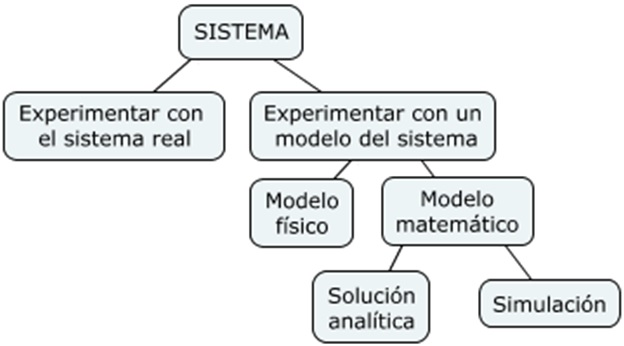
\includegraphics[width=7.5cm]{images/Sistema.jpg}
        \caption{Aproximaciones al estudio de un sistema}
        \label{fig:tipos_sol}
        %-------
        %Adapatado de LK
    \end{figure}
\end{frame}

\begin{frame}{Modelos}
    Un \textit{modelo} es definido como una representación de un sistema con el propósito de estudiarlo \cite{LK}.
\end{frame}

\begin{frame}{Tipos de Modelos}
    Los modelos pueden clasificarse de acuerdo con diferentes criterios:
    \begin{itemize}
        \item Matemáticos vs físicos.
        \item Estáticos vs dinámicos.
        \item Determinísticos vs estocásticos.
        \item Discretos vs continuos.
    \end{itemize}
\end{frame}